\documentclass{assignment}
\ProjectInfos{研究型物理实验}{PHYS1703}{2020-2021学年第一学期}{Note-3}{2020. 9. 25(周五)}{陈稼霖}{45875852}
\begin{document}
\section*{要求}
\begin{itemize}
    \item[(1)] 了解书本理论;
    \item[(2)] 了解Kramer-Kronig关系,并推导气体介质折射率实部与虚部(吸收率)之间的关系;
    \item[(3)] 完成书本习题I和II.
\end{itemize}

\section{气体折射率实部与虚部关系推导}
\subsection{经典方法}
将原子中的电子等效为由核束缚的谐振子,推导其在

无外场作用的情况下,原子中电子绕原子核运动,其平均位置$\bm{x}$与原子核位置(设为原点)重合,即$\bm{x}=0$;在弱场下,可近似认为电子平均位置的偏离正比场强,故可将电子等效为受原子核束缚的一个谐振子,其位移为电子平均位置相对于原子核的偏离$\bm{x}$,其本征振动频率$\omega_0$为电子在能级间跃迁的频率,其阻尼系数设为$\gamma$(在经典图像中无法得到阻尼系数的具体数值,只能通过实验得到经验值). 在一维情况下,该谐振子在电场$E(x,t)$中的动力学方程为
\begin{align}
    \label{motion-equ}
    m\ddot{x}=-eE(x,t)-\omega_0^2x-\gamma\dot{x},
\end{align}
其中上式右边三项分别为该谐振子受到的驱动力(电场力)、回复力和阻尼力.

对于真空中传播的电磁波,在空间中给定某点的电场可表为
\begin{align}
    E(t)=E_0e^{i\omega t}.
\end{align}
将其代入式\eqref{motion-equ}中,得
\begin{align}
    \label{motion-equ-2}
    m[\ddot{x}+\gamma\dot{x}+\omega_0^2x]=-eE_0e^{-i\omega t}.
\end{align}
从物理上看,谐振子应当和外加电场一样具有$\omega$的振荡频率,观察上面的微分方程,也不难猜到,上式的解应当有如下形式:
\begin{align}
    \label{trial-sol}
    x(t)=x_0e^{-i\omega t}.
\end{align}
将上式代入动力学方程式\eqref{motion-equ-2}中即可解得
\begin{align}
    x_0=-\frac{eE_0}{m}\frac{1}{(\omega_0^2-\omega^2)-i\gamma\omega}.
\end{align}
从而
\begin{align}
    x(t)=x_0e^{-i\omega t}=-\frac{eE(t)}{m}\frac{1}{(\omega_0^2-\omega^2)-i\gamma\omega}.
\end{align}

每个原子贡献的偶极矩为
\begin{align}
    p(t)=-ex(t)=\frac{e^2E(t)}{m}\frac{1}{(\omega_0^2-\omega^2)-i\gamma\omega}.
\end{align}
设气体中单位体积中有$N$个原子,则气体的电极化矢量为
\begin{align}
    P(t)=Np(t)=\frac{e^2NE(t)}{m}\frac{1}{(\omega_0^2-\omega^2)-i\gamma\omega}=\epsilon_0\chi E(t).
\end{align}
故电极化率为
\begin{align}
    \chi=\frac{e^2N}{\epsilon_0m}\frac{1}{(\omega_0^2-\omega^2)-i\gamma\omega}.
\end{align}
事实上,若仔细思考,上面得到的电极化率的表达式并非是完全准确的,例如,原子中往往存在不止一个电子,电子的有效电荷、有效质量也不一定是$e$、$m$(所幸的是,表达式的形式是没有错的,只是系数上存在一定偏差,我们将在下一小节尝试用量子力学的方法严谨地推导电极化率),故为了修正电极化率的表达式,我们引入一个经验系数$f$(又称振子强度),从而将电极化率表为
\begin{align}
    \chi=\frac{4\pi Nfe^2}{m}\frac{1}{(\omega_0^2-\omega^2)-i\omega\gamma}
\end{align}

作为非磁性介质,气体的折射率为
\begin{align}
    n=\sqrt{\epsilon_r}=\sqrt{1+\chi}.
\end{align}
对于较小的电极化率,上式可近似为
\begin{align}
    n\approx 1+\frac{\chi}{2}=1+\frac{2\pi Nfe^2}{m}\frac{1}{(\omega_0^2-\omega^2)-i\omega\gamma}=1+\frac{2\pi Nfe^2}{m}\frac{(\omega_0^2-\omega^2)+i\omega\gamma}{(\omega_0^2-\omega^2)^2+\omega^2\gamma^2}.
\end{align}
将折射率写成实部与虚部相加的形式
\begin{align}
    n=n_0(1+i\kappa),
\end{align}
则有
\begin{align}
    n_0=1-\frac{2\pi Nfe^2}{m}\frac{\omega^2-\omega_0^2}{(\omega^2-\omega_0^2)^2+\omega^2\gamma^2},
\end{align}
及
\begin{align}
    n_0\kappa=\frac{2\pi Nfe^2}{m}\frac{\omega\gamma}{(\omega^2-\omega_0^2)^2+\omega^2\gamma^2}.
\end{align}
当电磁场振荡频率与谐振子的本征频率相近(如本实验中入射激光的频率在铷原子共振频率附近扫描),$\omega\approx\omega_0$且$\omega-\omega_0\ll\gamma$,上面两式还可进一步近似为
\begin{align}
    n_0=&1-\frac{2\pi Nfe^2}{m}\frac{\frac{(\omega+\omega_0)(\omega-\omega_0)}{\omega_0(\omega+\omega_0)}}{\frac{(\omega+\omega_0)^2(\omega-\omega_0)^2+\omega^2\gamma^2}{\omega_0(\omega+\omega_0)}}\approx 1-\frac{2\pi Nfe^2}{m}\frac{(\omega-\omega_0)/\omega_0}{2(\omega-\omega_0)^2+\frac{1}{2}\gamma^2}=\frac{\pi Nfe^2}{m}\frac{\Delta\omega/\omega_0}{\Delta\omega^2+\gamma^2/4}.
\end{align}
和
\begin{align}
    n_0\kappa=\frac{2\pi Nfe^2}{m}\frac{\frac{\omega\gamma}{\omega_0(\omega+\omega_0)}}{\frac{(\omega+\omega_0)^2(\omega-\omega_0)^2+\omega^2\gamma^2}{\omega_0(\omega+\omega_0)}}\approx\frac{2\pi Nfe^2}{m}\frac{\frac{1}{2}\gamma/\omega_0}{2(\omega-\omega_0)^2+\frac{1}{2}\gamma^2}=\frac{\pi Nfe^2}{m}\frac{\gamma/2\omega_0}{\Delta\omega^2+\gamma^4/2}.
\end{align}

(TODO:为什么忽略电磁波中磁场造成的洛伦兹力的效果?需要估算和比较一下电场力和洛伦兹力的量级?)

\subsection{量子方法}
TODO:利用刘维尔-冯·诺依曼方程求解二能级系统得气体折射率实部与虚部关系

\section{Kramer-Kronig关系}
TODO...

\section{利用马赫-曾德尔干涉仪测量折射率与吸收率关系}
马赫-曾德尔(Mach-Zehnder,M-Z)干涉仪

\section{书本问题求解}
\begin{prob}
    Consider the photodiode output from the interferometer without the rubidium cell. Figure \ref{InterferometricOutputWithoutRbCell} shows the output at fixed laser frequency asa a function of $\Delta L$. The maxima in this are referred to as "fringes", from their spatial structure (which you will see in the lab when you set up the interferometer). How small must $\Delta L$ be in order for the photodiode output to go through less than one fringe as the laser is scanned over the rubidium resonance line (call it $5$ GHz)? To get the best results, you should try to set up your interferometer with $\Delta L$ less than this.
    \begin{figure}[h]
        \centering
        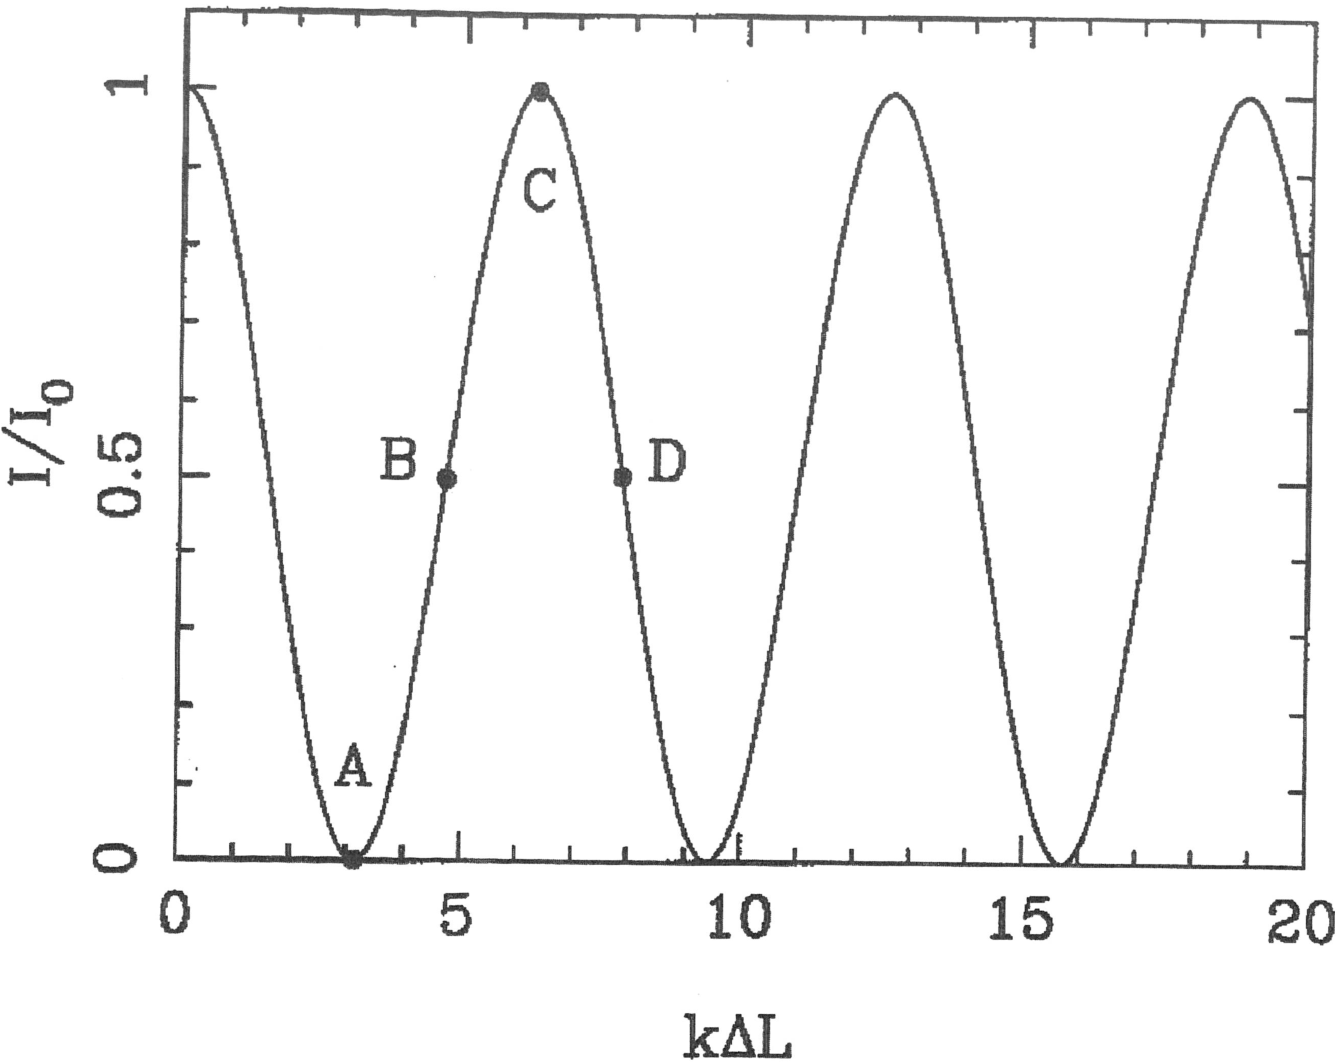
\includegraphics[width=.5\textwidth]{InterferometricOutputWithoutRbCell.png}
        \caption{Photodiode output vs. $k\Delta L$, where $k=\omega/c=2\pi/\lambda$, for a perfect Mach-Zehnder interferometer with no rubidium cell, at fixed laser frequency.}
        \label{InterferometricOutputWithoutRbCell}
    \end{figure}
\end{prob}
\begin{sol}
    为了使当激光扫过铷原子的共振频率范围($5$GHz)时光电探测器输出变化在一个fringe(即半个周期)以内,需要满足
    \begin{align}
        \Delta k\Delta L=\frac{2\pi\Delta\nu}{c}\Delta L=\frac{2\pi\times 5\times 10^9\text{Hz}}{3\times 10^8\text{m/s}}\Delta L\leq\pi,
    \end{align}
    即两条光路的光程差
    \begin{align}
        \Delta L\leq 3\times 10^{-2}\text{m}=3\text{cm}.
    \end{align}
\end{sol}

\begin{prob}
    Compute the photodiode output as a function of laser frequency around the rubidium resonance line, $I(\Delta\omega)/I_0$, for the set-up shown in Figure \ref{BasicSetup}. Assume the atoms in your cell are at rest (for ease of calculation) with some linewidth $\gamma$, so we can use the Lorentzian profile above for $\tau(\omega)$. Make three different plots of $I(\Delta\omega)/I_0$, one for each of three different values of the line center optical depth: $\tau_0=0.4$, $2$ and $20$. Make your plots over the range $-20\gamma<\Delta\omega<20\gamma$. Plot six curves on each plot, with values of $k\Delta L\mod(2\pi)$ equal to $j\pi/5$, with $j=0$ to $5$. The first and last of these correspond to the positions $A$ and $C$ in Figure \ref{InterferometricOutputWithoutRbCell}. Label your plots. You will be trying to reproduce these curves in the lab. (Check your calculations by comparing with the one calculated curve in Figure )
    \begin{figure}[h]
        \centering
        \includegraphics[width=.5\textwidth]{BasicSetup.png}
        \caption{The basic experiment set-up, consisting of a rubidium vapor cell in one arm of a Mach-Zehnder interferometer. The dotted line represent 50:50 beamsplitters. The input laser scans across the (Doppler broadened) rubidium absorption line.}
        \label{BasicSetup}
    \end{figure}
    \begin{figure}[h]
        \centering
        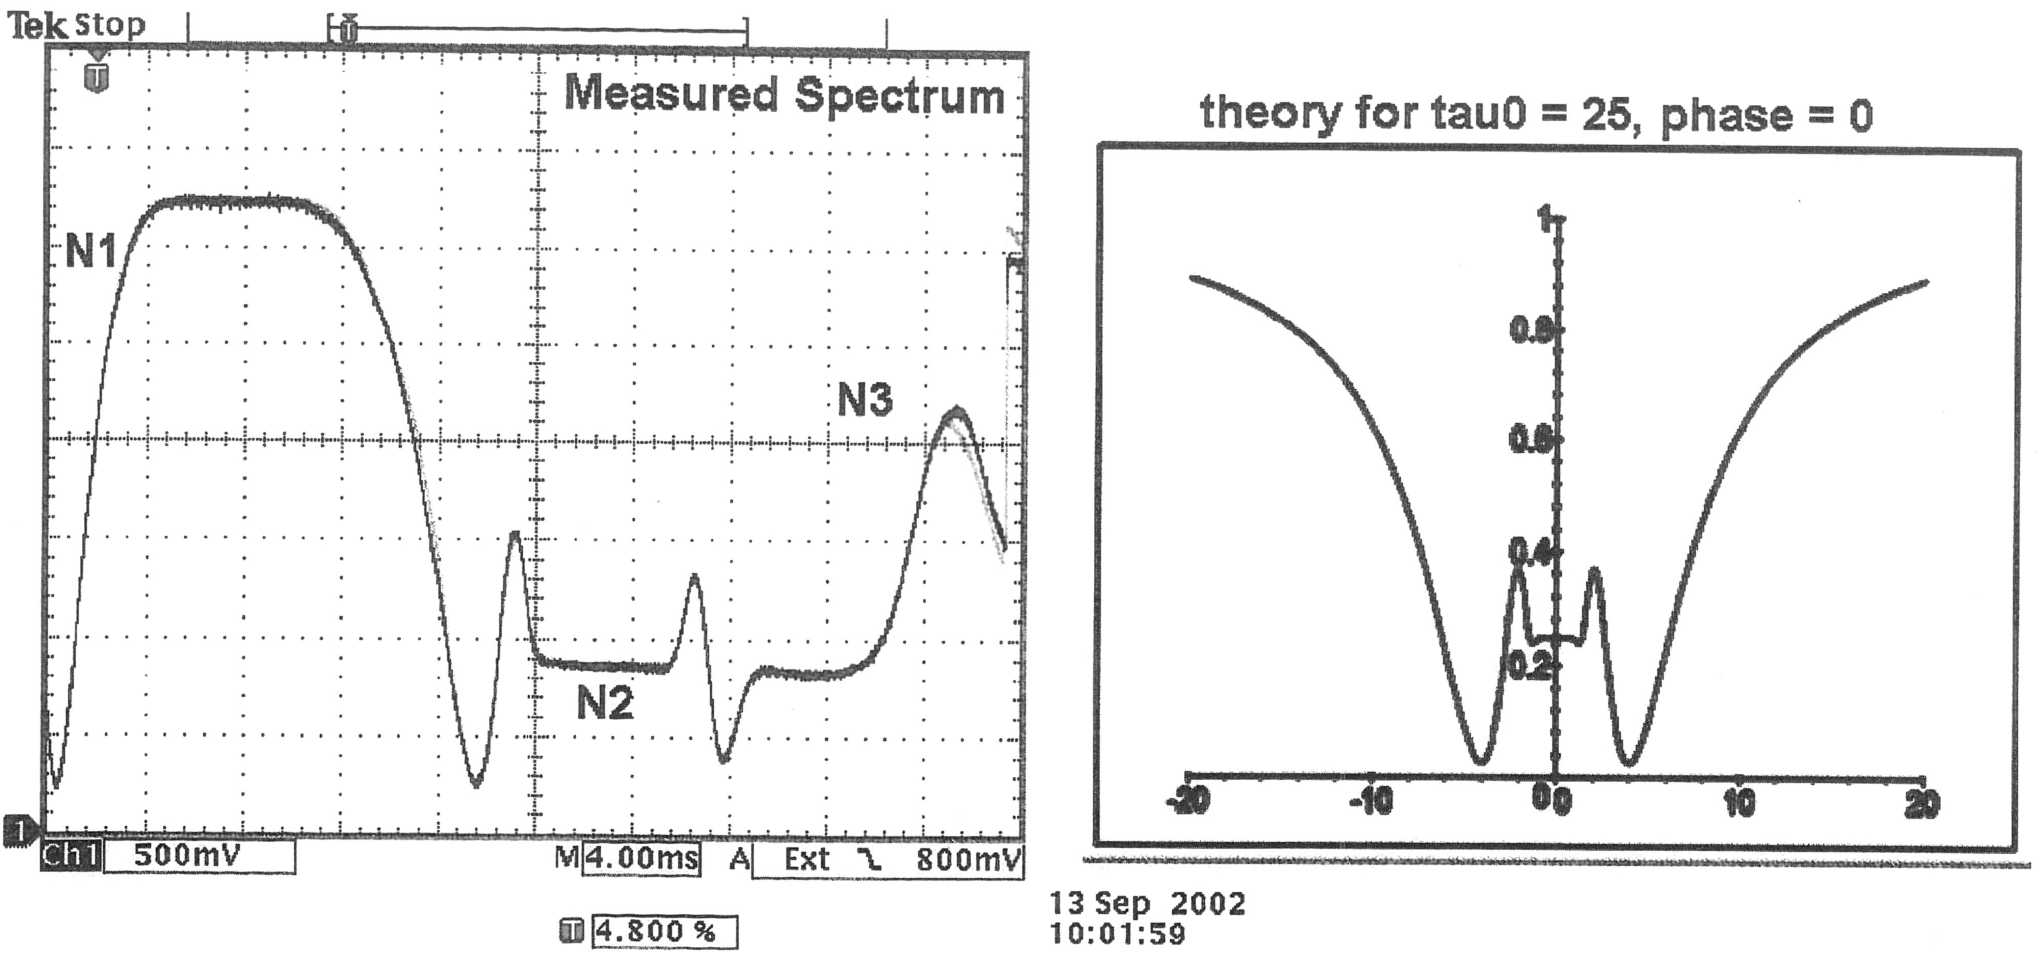
\includegraphics[width=.5\textwidth]{ComparisonOfMeasuredAndCalculatedSpectrum.png}
        \caption{A comparison of a measured spectrum (left) with a calculated spectrum (right). The plot shows $I(\Delta)/I_0$ versus $\Delta\omega/\gamma$. The calculation assumed $\tau=25$ at line center and $k\Delta L=0$. The measured spectrum is for the 85b line, but the adjacent 87b line complicates the right side of the spectrum (marked by N3). The center of the 85b line is at N2. The feature at N1 is an artifact of the laser scanning.}
    \end{figure}
\end{prob}
\begin{sol}
    当加入铷蒸汽腔,光电探测器的输出用频率可表为
    \begin{align}
        \frac{I(\Delta\omega)}{I_0}=\frac{1}{4}\left[1+e^{-2\tau}+2e^{-\tau}\cos\left(k\Delta L+\delta\right)\right].
    \end{align}
    其中
    \begin{align}
        \tau=&\frac{\tau_0\gamma^2}{\Delta\omega^2+\gamma^2},\\
        \delta=&k(n_0-1)\Delta z=\frac{(n_0-1)\tau}{\kappa}=-\frac{2\Delta\omega\tau}{\gamma}.
    \end{align}
\end{sol}
\end{document}